\chapter{Dados Reais} \label{cap:dadosreais}
\vspace{-2cm}

Durante o período de maio a julho de 2017 foram feitas aquisições de dados do detector para raios cósmicos, utilizando duas pás cintiladoras de dimensões $14$x$14$x$1$ posicionadas acima do plano superior do detector. A primeira pá foi posicionada a $4.5$ cm acima da superfície superior do detector enquanto a segunda pá foi posicionada a $47.5$ cm da mesma superfície.

Como as pás estão posicionadas para o céu, o sistema de \emph{trigger} foi configurado com o acionamento das duas pás para garantir um evento de raio cósmico.



\subsection{Metodologia de análise dos dados do experimento}

Os dados do experimento são salvos em arquivos de texto com o valor analógico da saída das PMTs convertido para digital (\ac{ADC}) podemos estimar a quantidade de \ac{p.e.} total de um evento estimando a contagem de ADCs no pico do evento, 


\subsection{Debug dos dados reais}

Devido à saturação das PMTs e da eletrônica de \emph{front-end}, os dados coletados com pico de energia acima do valor de saturação devem ser recuperados de alguma forma, foi utilizado um \emph{fitting} com uma forma do sinal conhecida através de um processo iterativo, calculando o erro provável de uma área linear pelo teste do $\chi^2$ (qui-quadrado, Apêndice \ref{apdx:qui-quadrado}) e utilizando a forma final com menor erro.

Após o \emph{fit} dos dados, foi encontrado um problema intrínseco ao método, como o \emph{fit} era realizado a partir do ponto de saturação eventos naquele ponto foram, em sua maioria, removidos do sistema como pode ser visto na Figura \ref{fig:peakdist_errado},  para resolver esste problema o \emph{fit} foi realizado a  partir de um ponto em que as PMTs não estão em saturação, gerando a Figura \ref{fig:peakdist}

\begin{figure}[H]
	\centering
	\hspace*{-2cm}
    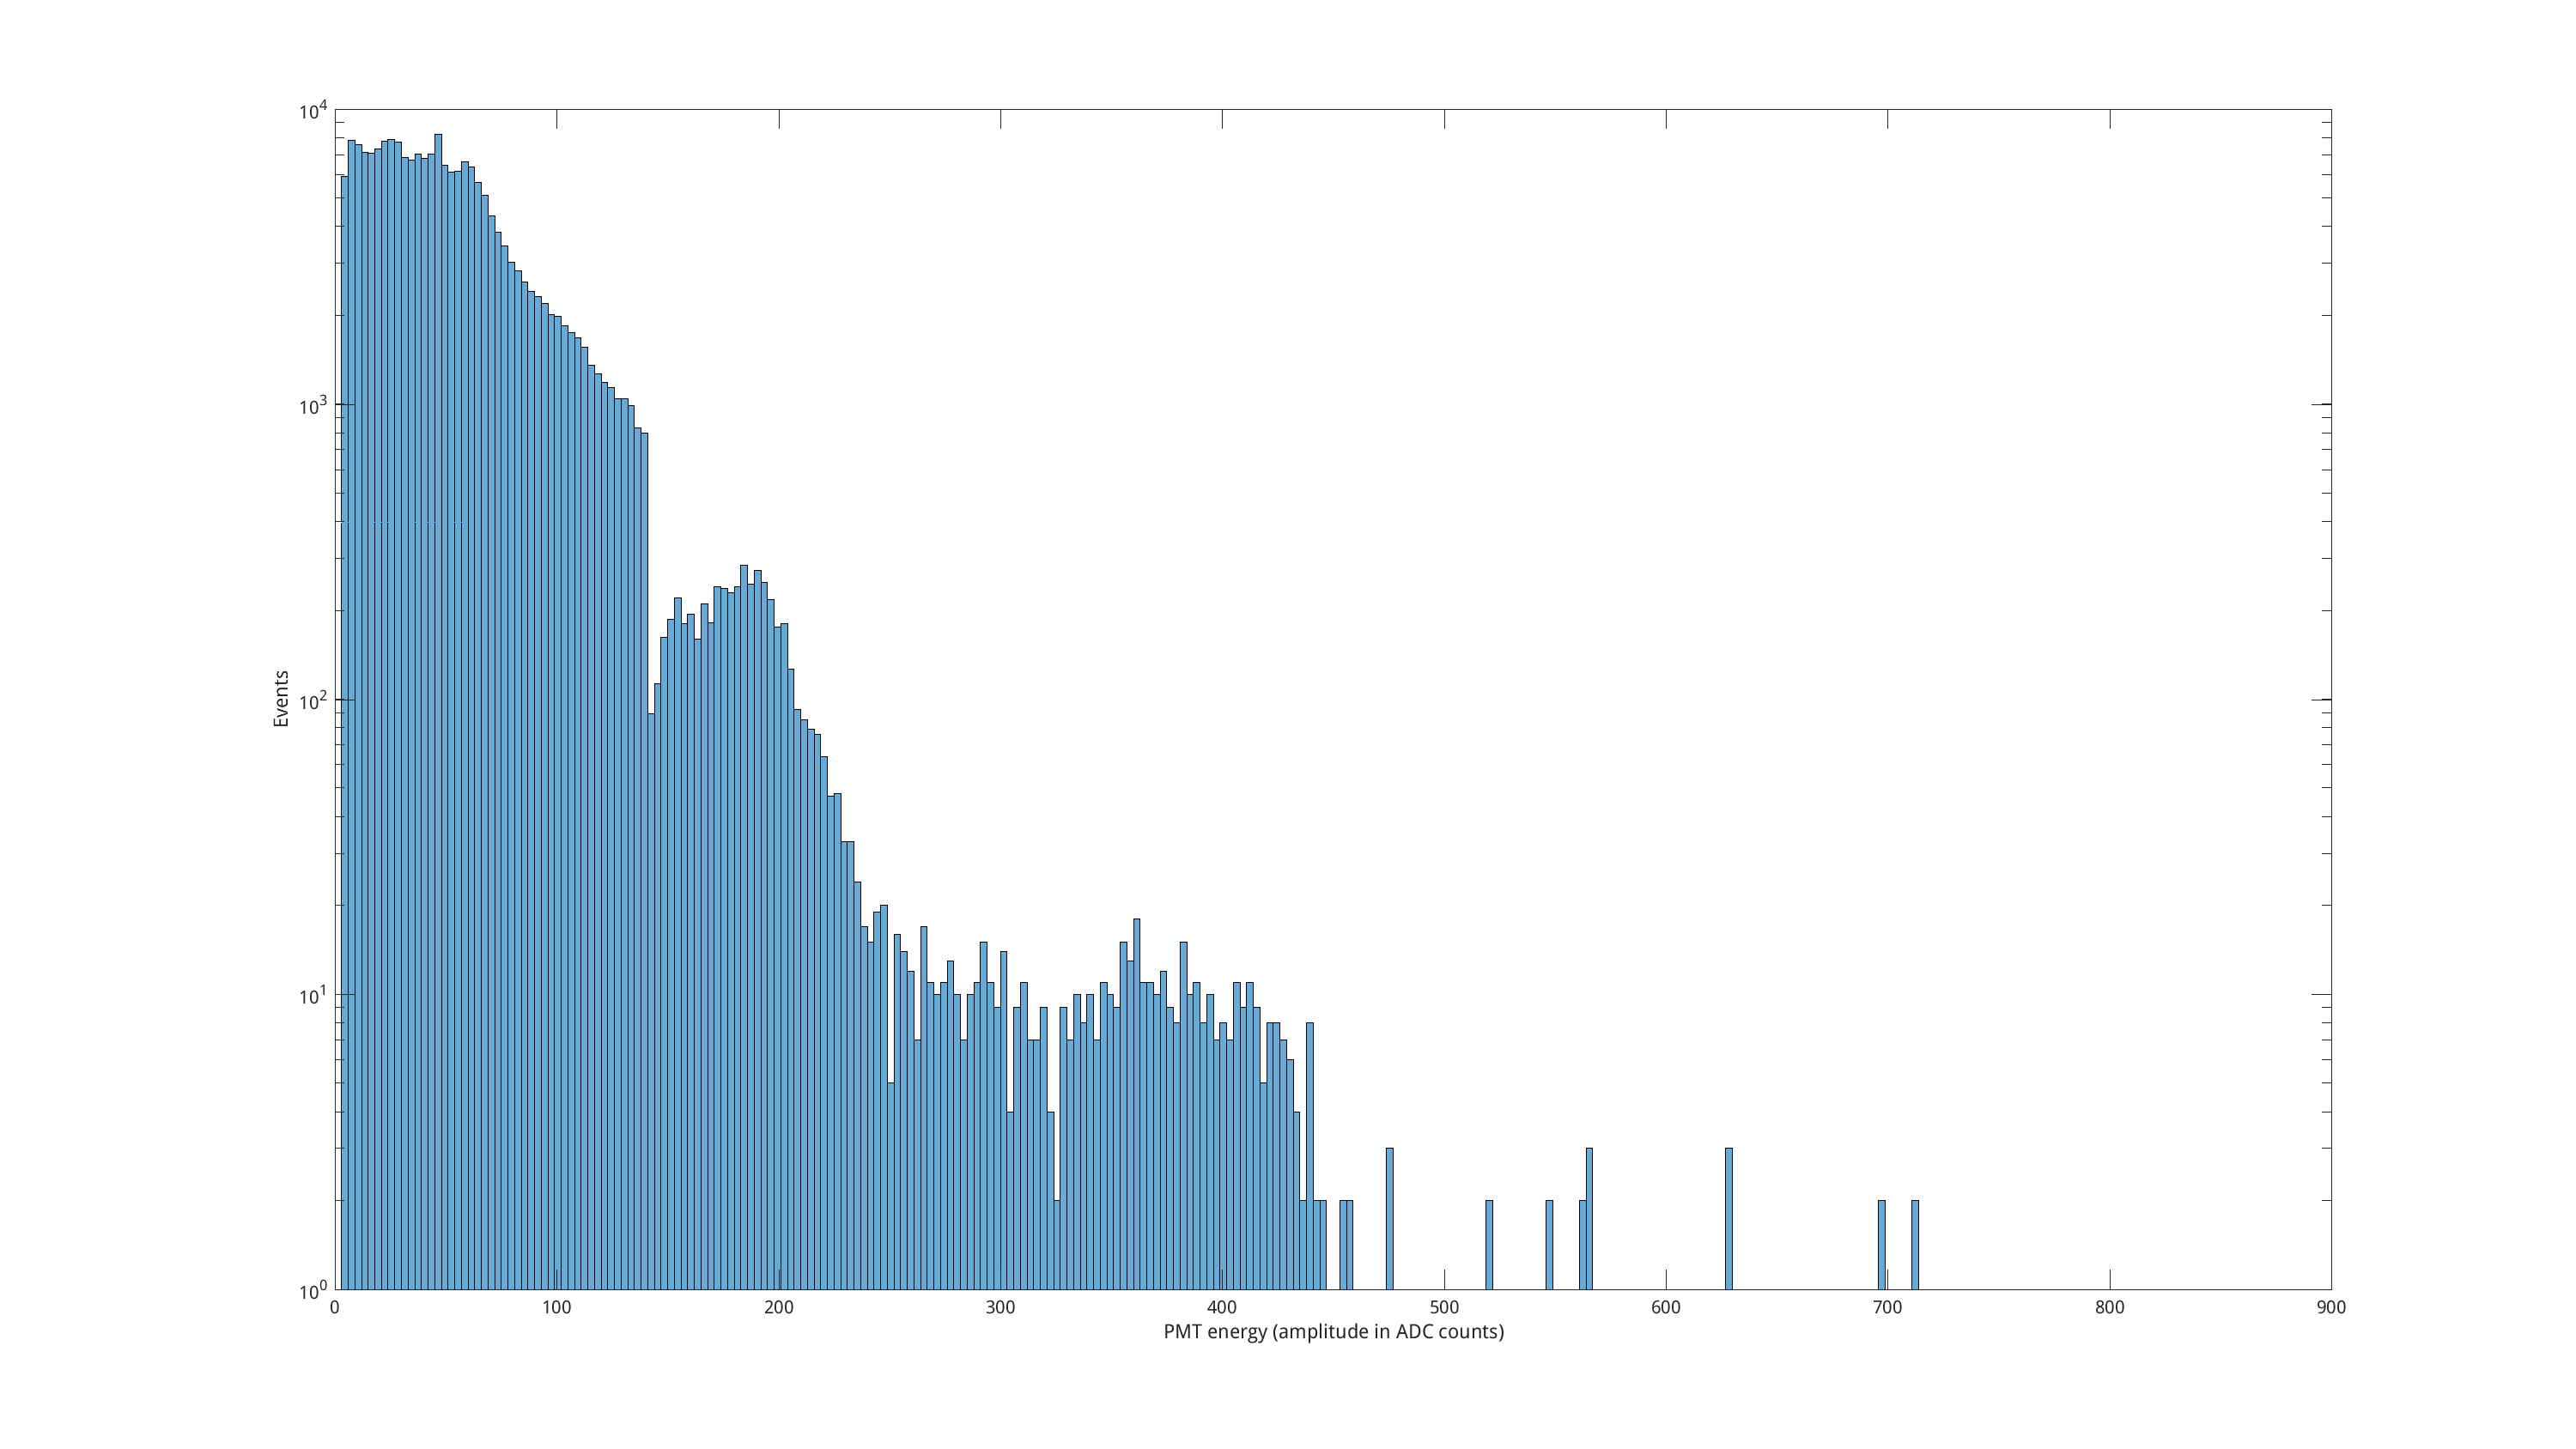
\includegraphics[width=19cm]{textuais/dadosreais/figuras/peakdist_errado.png}
	\caption{Distribuição de picos com problema causado pelo fit}
	\label{fig:peakdist_errado}
\end{figure}
\begin{figure}[H]
	\centering
	\hspace*{-2cm}
	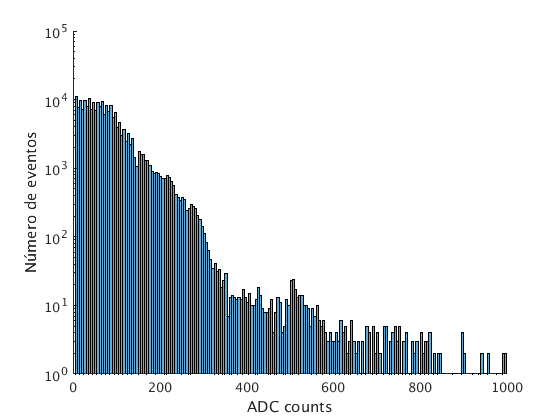
\includegraphics[width=19cm]{textuais/dadosreais/figuras/peakdist.png}
	\caption{Distribuição de picos após a resolução do problema do \emph{fit}}
	\label{fig:peakdist}
\end{figure}